\documentclass[12pt,oneside]{book}
\usepackage{geometry}                		% See geometry.pdf to learn the layout options. There are lots.
\geometry{a4paper}                   			% ... or a4paper or a5paper or ... 
%\geometry{landscape}                		% Activate for for rotated page geometry
%\usepackage[parfill]{parskip}    		% Activate to begin paragraphs with an empty line rather than an indent
\usepackage{graphicx}				% Use pdf, png, jpg, or epsß with pdflatex; use eps in DVI mode
								% TeX will automatically convert eps --> pdf in pdflatex		
\usepackage{amssymb}

\usepackage[spanish]{babel}			% Permite que partes automáticas del documento aparezcan en castellano.
\usepackage[utf8]{inputenc}			% Permite escribir tildes y otros caracteres directamente en el .tex
\usepackage[T1]{fontenc}				% Asegura que el documento resultante use caracteres de una fuente apropiada.

\usepackage{hyperref}				% Permite poner urls y links dentro del documento

\title{SUDOKU \\ Manual de Usuario}
\author{José Velez \\ Diego Cabrera \\ Carlos Ramirez}
%\date{}							% Activate to display a given date or no date

\begin{document}
\maketitle
\tableofcontents

\chapter{Derechos del Autor}
La aplicacion que simula el Juego de Sudoku fue creada por propositos academicos como proyecto del Primer Parcial de la materia de Lenguajes de Programación que dicta el Ing. Tibau en el presente semestre I Termino-2013, el uso de esta aplicación es de uso gratiuto por cualquier usuario, sin embargo su codigo fuente no puede ser usado por ninguna persona a excepcion de los 3 estudiantes autores del Proyecto.

\chapter{Prefacio}

Este manual de usuario pretende brindar un conjunto de instrucciones al Usuario para facilitar el funcionamiento del juego SUDOKU. \ \\ \\ 
Por otro lado, también brinda guías para el juego y describe las diferentes instancias que tiene el mismo. \ \\ \\
Con el fin de aprovechar al máximo la información de este documento, para ejecutar la aplicación de SUDOKU el usuario debe tener en su poder un PC que tenga instalado un Sistema Operativo Windows (XP, Vista, 7) o Linux (preferible UBUNTU).

\chapter{Introducción}

El Sudoku  fue creado en 1979 por Howard Garns un arquitecto de primera y publicado en una revista de Rompecabezas Americano. El golpe moda en Japón fue en 1986, pero no tomaron el centro de la escena hasta el 2005, cuando sitios web, libros rompecabezas y la cobertura de los medios de comunicación, hicieron que  significativos juego de Sudoku se convirtieran en una sensación mundial.

\chapter{Reglas del Juego}
El juego está compuesto por una cuadrícula de 9x9 casillas, partiendo de algunos números ya dispuestos en algunas de las casillas, hay que completar las casillas vacías con dígitos del 1 al 9 sin que se repitan por fila, columna o región. \\ \\ Regla 1: Completar las casillas vacías con un solo número del 1 al 9. \\ Regla 2: En una misma fila no puede haber números repetidos. \\ Regla 3: En una misma columna no puede haber números repetidos. \\ Regla 4: En una misma región no puede haber números repetidos. \\ Regla 5: la solución de un sudoku es única.

\begin{figure}[htbp]
\begin{center}
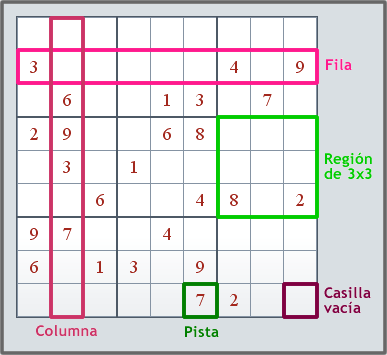
\includegraphics[width=.50\textwidth]{./imagenes/Reglas.png}
\caption{Reglas de Juego}
\label{Reglas}
\end{center}
\end{figure}

\chapter{Guía del Juego}

\section{Inicio}

Para iniciar la aplicacion de Sudoku se debe dar click al boton ENTRAR.

\begin{figure}[htbp]
\begin{center}
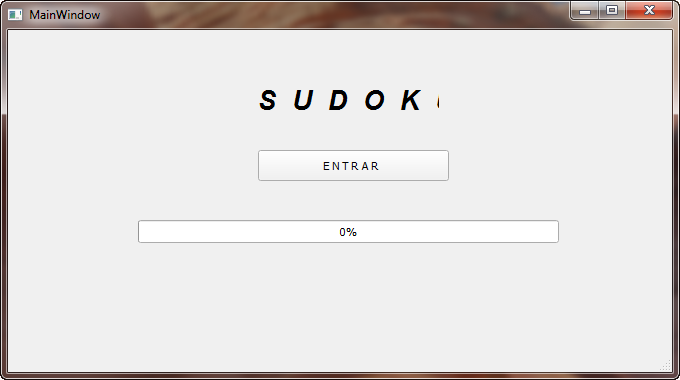
\includegraphics[width=.60\textwidth]{./imagenes/Inicio.png}
\caption{Inicio}
\label{Inicio}
\end{center}
\end{figure}

Luego nos aparece la siguiente ventana, donde se podrá escoger diversidad de opciones para poder jugar partidas de Sudoku.

\begin{figure}[htbp]
\begin{center}
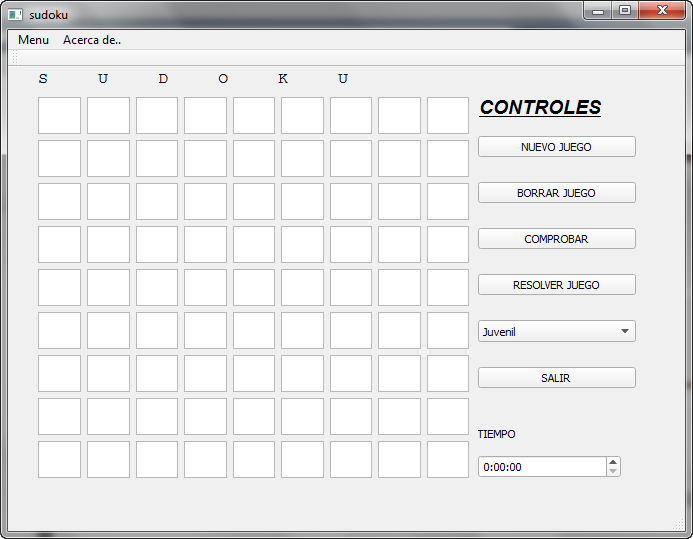
\includegraphics[width=.60\textwidth]{./imagenes/Menu.png}
\caption{Inicio}
\label{Inicio}
\end{center}
\end{figure}

 

\section{Controles}

\begin{figure}[htbp]
\begin{center}
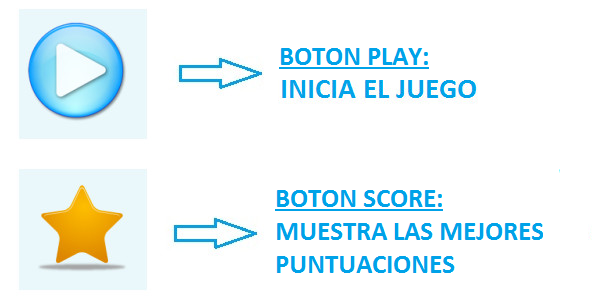
\includegraphics[width=.40\textwidth]{./imagenes/Controles.png}
\caption{Controles}
\label{Controles}
\end{center}
\end{figure}


\begin{center}
\textbf{NUEVO JUEGO} 
\\ Inicia una nueva partida en cualquier instancia del Juego.
\ \\ \ \\

\textbf{BORRAR JUEGO} 
\\ Elimina el contenido de todas las casillas. \ \\ \ \\

\textbf{COMPROBAR} 
\\ Verifica si la solución propuesta por el usuario esta correcta o incorrecta. 
\ \\ \ \\

\textbf{RESOLVER JUEGO}  
\\ Muestra la solución del SUDOKU. 
\ \\ \ \\

\textbf{SALIR}  
\\ Cierra la aplicación. 
\ \\ \ \\ 

\textbf{GUARDAR PARTIDA}  
\\ Guarda una partida iniciada. 
\ \\ \ \\ 

\textbf{CARGAR PARTIDA}  
\\ Carga una partida que ha sido guardada. 
\ \\ \ \\ 

\textbf{ALERTA DE JUGADAS INVALIDAS}  
\\ Muestra una alerta cuando se digita un valor incorrecto en alguna casilla. 
\ \\ \ \\ 

\textbf{ALERTA DE JUGADAS INCORRECTAS}  
\\ Muestra una alerta en todas las casillas que tienen valores incorrectos. 
\ \\ \ \\ 

\textbf{SCORE DE PARTIDAS}  
\\ Visualiza las mejores partidas. 
\ \\ \ \\ 

\textbf{DIFICULTAD} 
\\ Consta de 3 niveles.
\end{center}

\begin{figure}[htbp]
\begin{center}
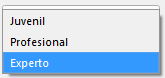
\includegraphics[width=.20\textwidth]{./imagenes/Nivel.png}
\caption{Niveles de Dificulatad}
\label{Niveles de Dificulatad}
\end{center}
\end{figure}

\begin{center}
Seleccionando la opción \textbf{MENU -> QUIT} (Figura 5.5) también podemos cerrar la aplicación y al seleccionar la opción \textbf{ACERCA DE.. -> HELP} (Figura 5.6) obtenemos información de la aplicación.
\end{center}

\begin{figure}[htbp]
\begin{center}
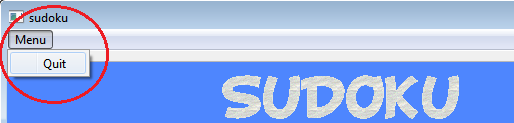
\includegraphics[width=.15\textwidth]{./imagenes/SeleccionMenu.png}
\caption{Opción Menu}
\label{Opcion Menu}
\end{center}
\end{figure}

\begin{figure}[htbp]
\begin{center}
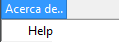
\includegraphics[width=.15\textwidth]{./imagenes/SeleccionAcerca.png}
\caption{Opción Acerca de..}
\label{Opcion Acerca de..}
\end{center}
\end{figure}





\section{JugandoSudoku}

1. Al iniciar la aplicación la tabla de Sudoku aparece encerada, de la siguiente manera:

\begin{figure}[htbp]
\begin{center}
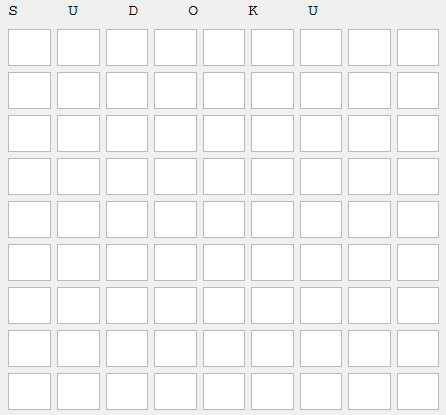
\includegraphics[width=.42\textwidth]{./imagenes/Tabla.png}
\caption{Tabla}
\label{Tabla}
\end{center}
\end{figure}


2. Para empezar una nueva partida, primero escogemos el nivel de dificultad (Figura 5.4), luego escogemos la opción NUEVO JUEGO (Figura 5.3). \\ Entonces nos aparecerá la tabla de Sudoku con celdas resueltas y celdas vacías (Dependiendo del Nivel de Dificultad aparacerán menos casillas vacías si el nivel escogido es Juvenil, y más casillas vacias si el nivel es más avanzado).


\begin{figure}[htbp]
\begin{center}
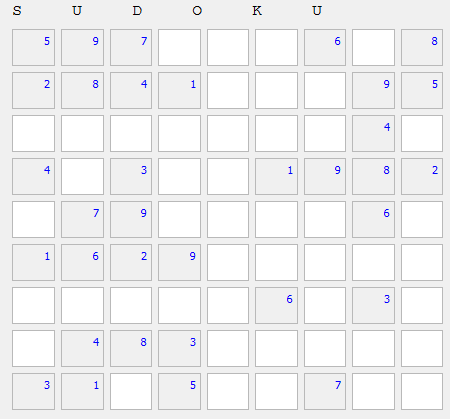
\includegraphics[width=.42\textwidth]{./imagenes/Tabla1.png}
\caption{Tabla1}
\label{Tabla1}
\end{center}
\end{figure}


3. Mientras se esta resolviendo alguna partida de SUDOKU se podrán realizar diversidad de acciones dependiendo de las opciones que vaya escogiendo el usuario: 

\begin{center}
- Si escogemos la opción BORRAR JUEGO (Figura 5.3), la tabla del Sudoku se encera (Figura 5.7). 
\ \\ \ \\ 

- Si escogemos la opcion NUEVO JUEGO (Figura 5.3)  se borrá el avance de la solución actual propuesta por el usuario y se inicia una nueva partida (Figura 5.8). 
\ \\ \ \\ 

- Si seleccionamos la opción de ALERTA DE JUGADA INVALIDA, cada vez que digitemos un valor incorrecto la aplicación mostrará una alerta, mientras que si seleccionamos la opcion ALERTA DE JUGADAS INCORRECTAS, la aplicación nos mostrará alertas en todas las casillas en que este un valor incorrecto de la siguiente manera:
\end{center} 
 
\begin{figure}[htbp]
\begin{center}

\includegraphics[width=.60\textwidth]{./imagenes/NoDisponible.png}
\caption{ImagenPendiente}
\label{ImagenPendiente}
\end{center}
\end{figure}

\begin{center}
- En cualquier instancia de la partida podemos guardar la partida o cargar una partida que ha sido anteriormente guardada. 
\ \\ \ \\ 

- Si queremos visualizar la solución del Juego, seleccionamos la opción RESOLVER JUEGO (Figura 5.3) y la aplicación muestra la solución del Juego y la partida termina.
\end{center} 

\begin{figure}[htbp]
\begin{center}
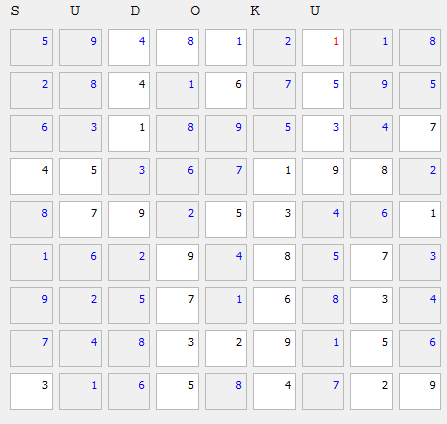
\includegraphics[width=.50\textwidth]{./imagenes/JuegoResuelto.png}
\caption{Juego Resuelto}
\label{Juego Resuelto}
\end{center}
\end{figure}

4. Si hemos terminado de resolver la partida por nuestra cuenta, procedemos a seleccionar lo opción COMPROBAR (Figura 5.3) y dependiendo de que si la solución es correcta o incorrecta la aplicación mostrará el siguiente mensaje:

\begin{figure}[htbp]
\begin{center}

\includegraphics[width=.50\textwidth]{./imagenes/NoDisponible.png}
\caption{ImagenPendiente}
\label{ImagenPendiente}
\end{center}
\end{figure}

\ \\ \ \\ \ \\ \ \\

5. Por último si deseamos observar las mejores partidas jugadas procedemos a seleccionar la opción SCORE DE PARTIDAS.

\begin{figure}[htbp]
\begin{center}

\includegraphics[width=.50\textwidth]{./imagenes/NoDisponible.png}
\caption{ImagenPendiente}
\label{ImagenPendiente}
\end{center}
\end{figure}




\chapter{Preguntas Frecuentes}

\begin{center}

\textbf{¿Puedo subir de nivel mientras estoy jugando una partida?} \\ No, el nivel se escoge antes de iniciar la partida, por lo que se debería iniciar una partida nueva para subir ó bajar un nivel de dificultad.
\ \\ \ \\ \ \\

\textbf{¿Al escoger la opción salir mientras estoy jugando una partida, la partida se guarda automaticamente?} \\ No, una partida solo se guarda al seleccionar la opción GUARDAR PARTIDA.
\ \\ \ \\ \ \\

\textbf{¿Si escojo la opción borrar juego, se borran solo las casillas que he resuelto?} \\ Al seleccionar esta opción se borra el contenido de todas las 81 casillas, las propuestas y las resueltas.
\ \\ \ \\ \ \\

\textbf{¿Puedo parar el tiempo en algún instante de la partida?} \\ No, el tiempo se inicia automaticamente cuando se inicia la partida y solo se detiene al finalizar la misma.


\end{center}

\chapter{Glosario}
\ \\
\textbf{NIVEL:} \\ El juego se subdivide en 3 niveles que diferencian la dificultad que tiene cada partida.
\ \\ \ \\ 
\textbf{PARTIDA:} \\ Flujo del juego en donde el objetivo es resolver una tabla de Sudoku llenando las casillas vacias de la tabla con numeros del 1 al 9.
\ \\ \ \\ 
\textbf{CASILLA:} \\Son las 81 celdas que conforman la tabla 9x9 del Sudoku.
\ \\ \ \\ 
\textbf{CARGAR:} \\ Abre nuevamente una partida anteriormente guardada.
\ \\ \ \\
\textbf{SCORE:} \\ Listado con las mejores puntuaciones de las partidas jugadas.


\end{document}  
